\section{Solucion}
\subsection{Objetivo}
\begin{frame}[shrink]
  \frametitle{Objetivo}
  Como respuesta a la situación actual, se define el siguiente objetivo:
  \begin{block}{Objetivo}
    Construir una solución de software libre con capacidades de WAF y aceleración SSL/TLS, que sea  fácilmente desplegable y que minimice el esfuerzo y el impacto que dicha
    solución tiene sobre la plataforma web actual o futura.
    \par También debe ser fácilmente adaptable a diferentes necesidades y entornos.
  \end{block}
\end{frame}

\subsection{Diseño}
\begin{frame}[shrink]
  \frametitle{Diseño}
  \begin{figure}
    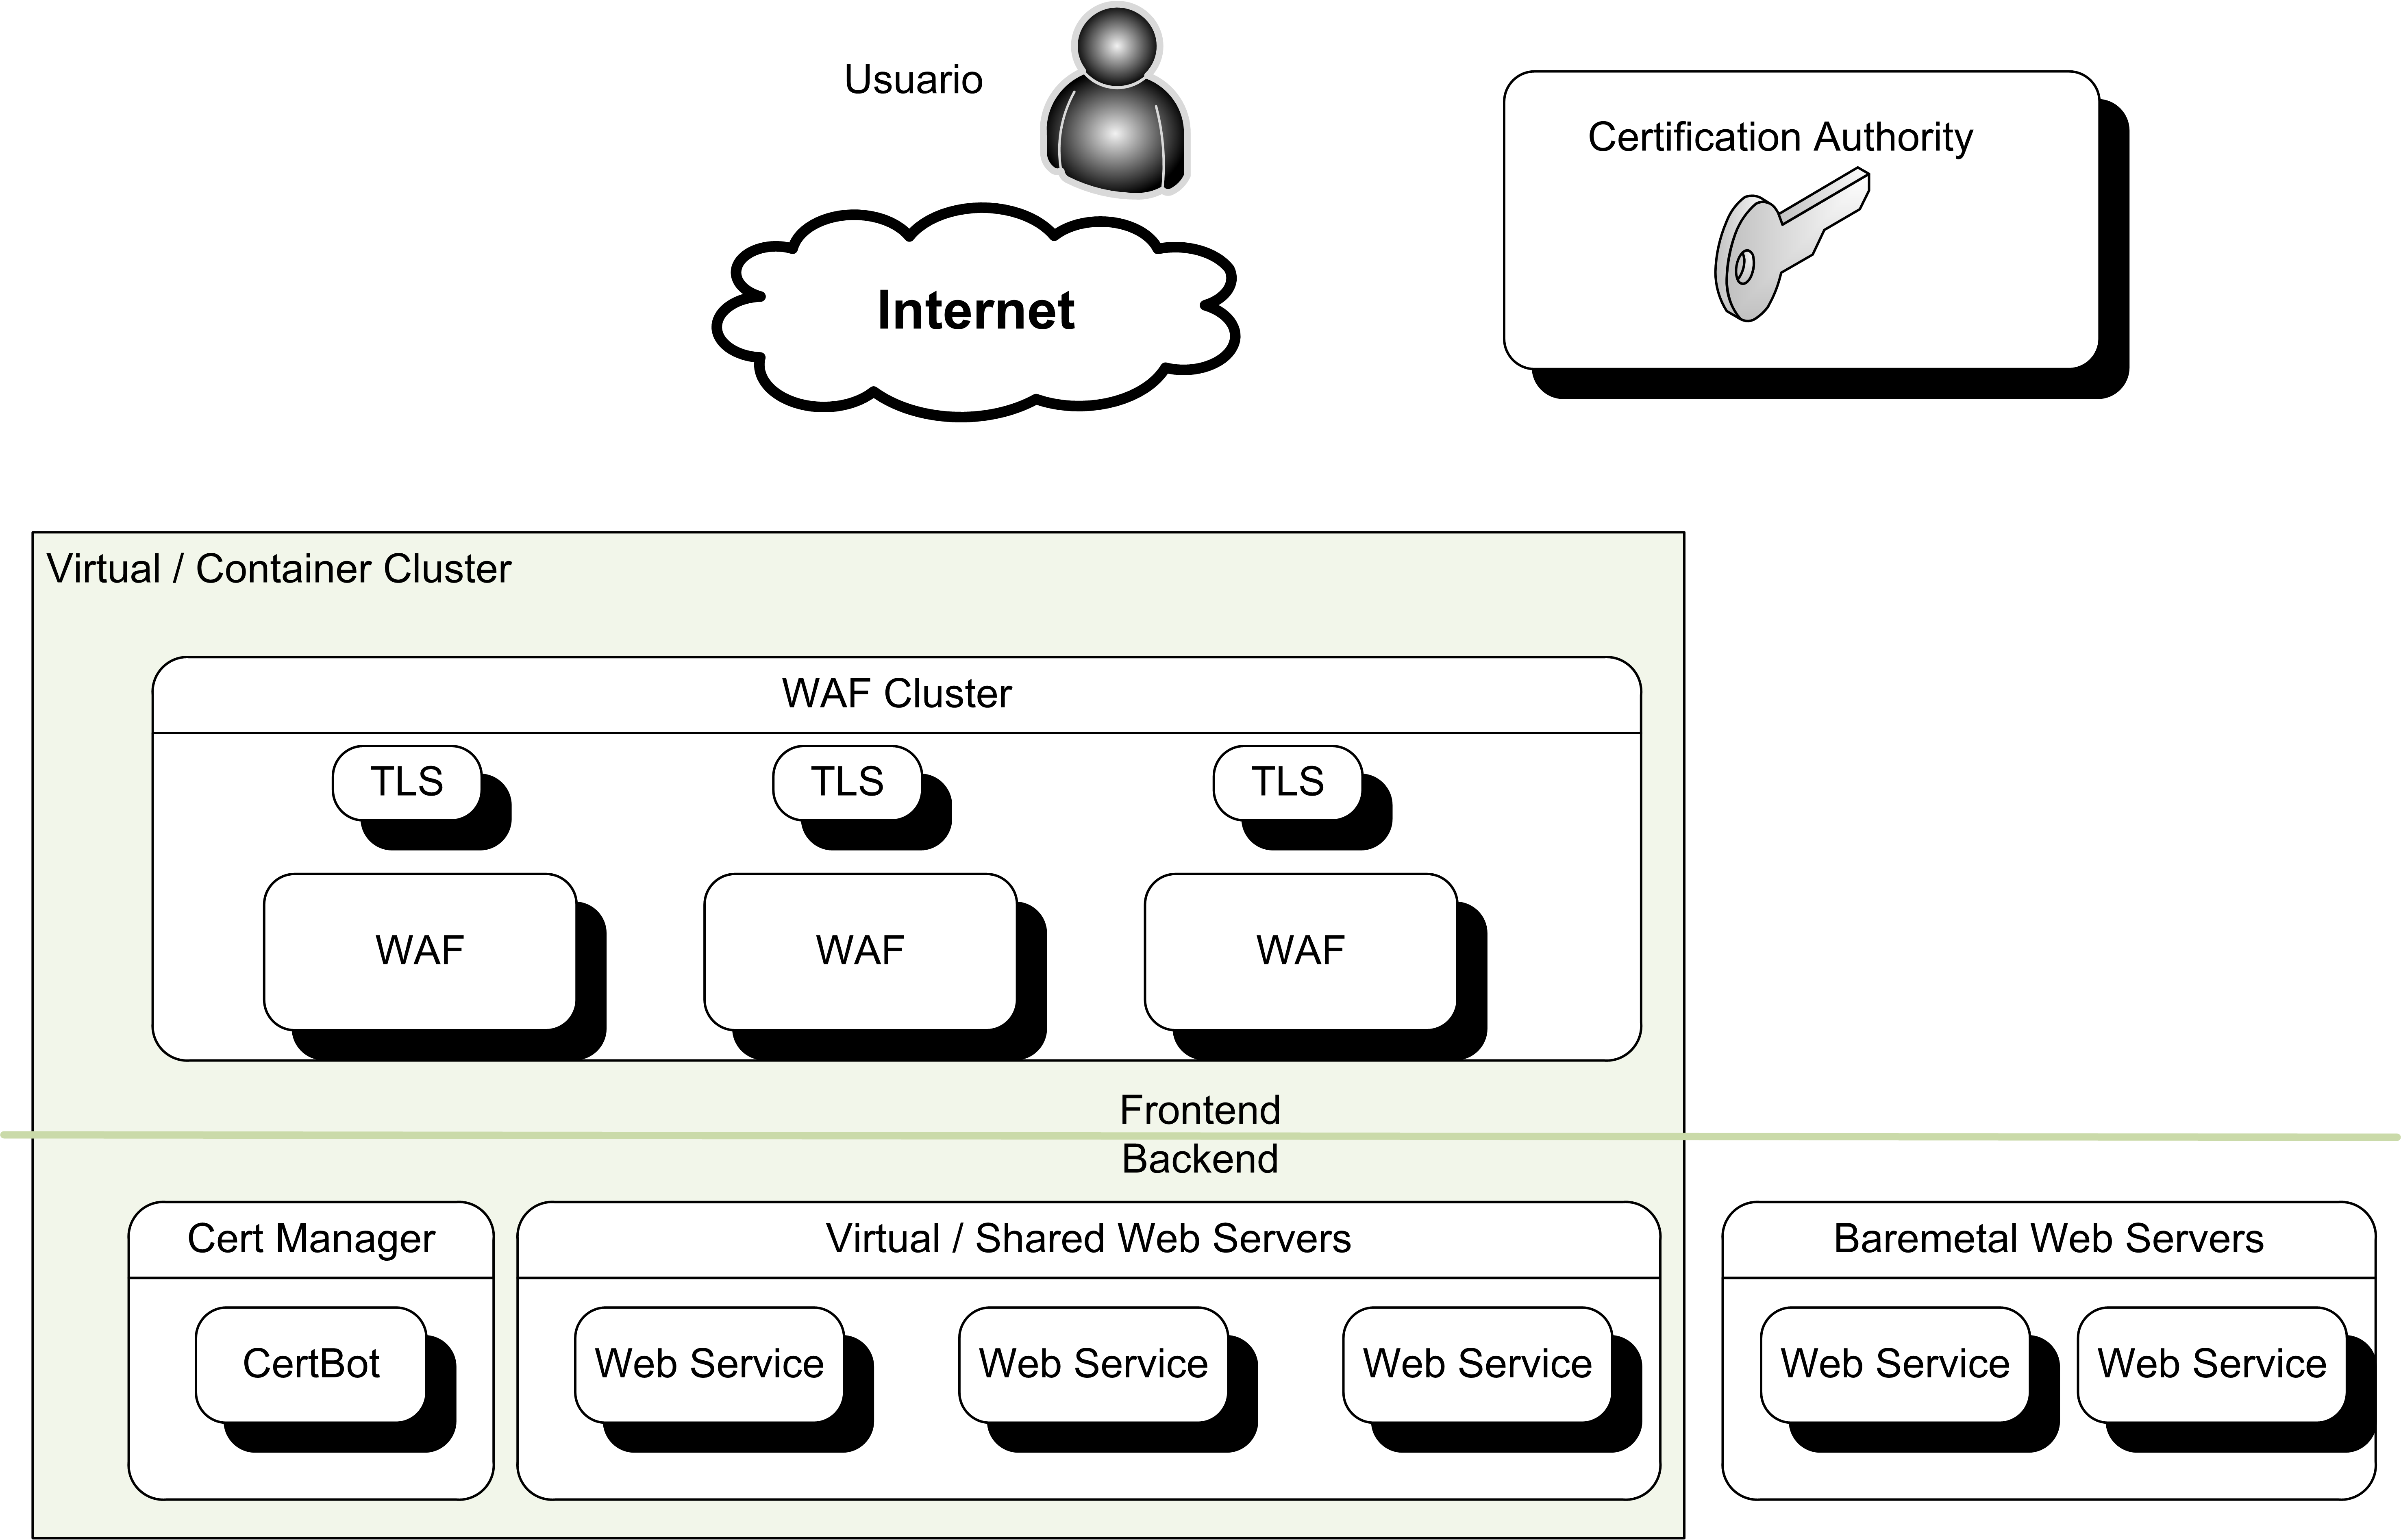
\includegraphics[width=0.9\textwidth]{fig/Diagram_HLD}
    \caption{\small{Diseño a alto nivel de la solución}}
  \end{figure}
\end{frame}

\begin{frame}[shrink]
  \frametitle{Componentes}
  \begin{itemize}
    \item WAF.
    \item Software criptográfico.
    \item Software de virtualización.
    \item Software de orquestación.
    \item Software de aprovisionamiento y gestión de certificados.
    \item Servicio de almacenamiento.
    \item Políticas de auditoría y controles de seguridad.
  \end{itemize}
\end{frame}

\subsection{Arquitectura}
\begin{frame}[shrink]
  \frametitle{Arquitectura}
  \begin{figure}
    \includegraphics[width=0.9\textwidth]{fig/Diagram_Complete_LLD}
  \end{figure}
\end{frame}

